\newpage
\subsection{Implementing invert}
\visHeader
\hypertarget{invertCard vis}{}

\begin{itemize}

% Make sure you explain how/why the green box. Hasn't been convered yet
\item[$\blacktriangleright$] Model the SDM depicted in Fig.~\ref{fig:sdm_invert}. Remember, the green creational object variable is made by setting the binding
operator as \texttt{create}.

% Explain how to use the new assignments??

\vspace{1cm}

\begin{figure}[htbp]
\begin{center}
  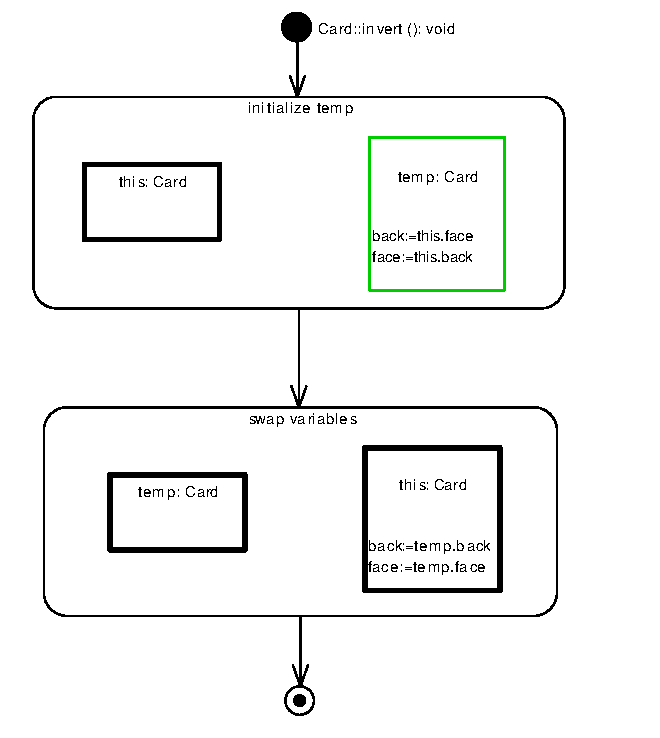
\includegraphics[width=0.9\textwidth]{ea_swappingCard.pdf}
  \caption{Swap back and face of the card}  
  \label{fig:sdm_invert}
\end{center}
\end{figure}

\item[$\blacktriangleright$] Believe or not, that's it! Check out how this method was implemented in the textual syntax by reviewing
Fig.~\ref{fig:invertPatterns} in the next section.

\end{itemize}
